% !Mode::"TeX:UTF-8"
\documentclass[twocolumn,landscape,UTF8]{ctexart}
\include{package}
%\usetag{ans}             % 注释掉该行语句不显示答案
%\usetag{kai}             % 注释掉改行语句为闭卷
\begin{document}
\newcommand{\school}{中国计量大学}
\def\kecheng{高等数学A1}   % 课程名称
\def\xueniana{19}         % 学年始
\def\xuenianb{20}         % 学年终
\def\xueqi{1}             % 学期
\def\leixing{A}           % 试卷类型
\def\kaikexueyuan{理学院}  % 开课学院
\def\class{重修班}         % 学生班级
\def\teacher{何足道}       % 教师
\def\nian{2020}           % 考试时间 年
\def\yue{01}              % 考试时间 月
\def\ri{04}               % 考试时间 日
\def\shi{9}               % 考试时间 时
\def\ruchang{证件、文具等考试必备物品}  % 允许带入考场的物品
\fancyhead[LO]{\iftagged{ans}{}{\begin{tabular}{|m{1.2cm}|m{5mm}|}\hline
		\raisebox{-0.5ex}{座位号} &	\\[0.5ex]\hline
\end{tabular}}}
\fancyfoot[CO,CE]{\vspace*{1mm}\small%
	\school20\underline{\xueniana}$\sim$20\underline{\xuenianb}\,学年第\underline{\xueqi}学期{《\kecheng》}\iftagged{ans}{试卷(\leixing)参考答案和评分标准}{课程考试试卷(\leixing)}第\underline{\stepcounter{mypage}\themypage}页,共\underline{\themylastpage}页 \hspace{1.5cm}
	\school20\underline{\xueniana}$\sim$20\underline{\xuenianb}\,学年第\underline{\xueqi}学期{《\kecheng》}\iftagged{ans}{试卷(\leixing)参考答案和评分标准}{课程考试试卷(\leixing)}第\underline{\stepcounter{mypage}\themypage}页, 共\underline{\themylastpage}页}%\pageref{LastPage}
\sbox{\zdx}
{\parbox{27cm}{\centering
%	座位号~\underline{\makebox[34mm][c]{}}~ 班~级\underline{\makebox[34mm][c]{}}~\CJKfamily{song} 学~号\underline{\makebox[44mm][c]{}}~\CJKfamily{song} 姓~名\underline{\makebox[34mm][c]{}} ~\\
%	\vspace{3mm}
%请在所附答题纸上空出密封位置。并填写试卷序号、班级、学号和 姓名\\
%%答题时学号
\vspace{1cm}
\dotfill{} 密\dotfill{}封\dotfill{}线\dotfill{} \\
	}}
\reversemarginpar
	
\begin{spacing}{1.25}
	\begin{center}
\begin{LARGE}
{\heiti\school~20\underline{\xueniana}~$\sim$~20\underline{\xuenianb}\,学年~第\,\underline{~\xueqi~}\,学期\\
{《~\kecheng~》}\,\iftagged{ans}{试卷(\leixing)参考答案和评分标准}{课程考试试卷(~\leixing~)}}\\
\end{LARGE}
\end{center}
%(闭卷笔试\ \ 90 分钟)\\
	\vspace{0.5cm}

\iftagged{ans}{\noindent 开课二级学院:\underline{\makebox[2cm][c]{\kaikexueyuan}},学生班级:\underline{\makebox[4cm][c]{\class}},教师:\underline{\makebox[2cm][c]{\teacher}}}%
{开课二级学院:\underline{\makebox[3cm][c]{\kaikexueyuan}},考试时间:\underline{~\nian~}年\underline{~\yue~}月\underline{~\ri~}日\underline{~\shi~}时

 考试形式:{闭卷{\raisebox{0.5ex}{\scalebox{0.8}[0.6]{\fbox{\iftagged{kai}{\color{white}}{}$\surd$}}}}、开卷{\raisebox{0.5ex}{\scalebox{0.8}[0.6]{\fbox{\iftagged{kai}{}{\color{white}}$\surd$}}}}},允许带\underline{\makebox[6.5cm][c]{\ruchang}}入场
 
 考生姓名:\underline{\hspace{2cm}} 学号:\underline{\hspace{2cm}} 专业:\underline{\hspace{2cm}} 班级:\underline{\hspace{1.5cm}} 

%\vspace{0.25cm}
\begin{center}
\begin{tabular}{|>{\centering\arraybackslash}m{0.0385\textwidth}|*{7}{>{\centering\arraybackslash}m{0.035\textwidth}|}}
	\hline
题~序 & 一 &  二 & 三 & 四 & 五 & 六 & 总~分  \\\hline
得~分 &  &  &  &  &  &  &   \\\hline
评卷人 &  &  &  &  &  &  &   \\\hline
\end{tabular}
\end{center}
}
\end{spacing}
\vspace{-0.5cm}
\setlength{\marginparsep}{1.7cm}
\iftagged{ans}{}{\putzdx} %%装订线--奇页数
\vspace{1cm}

%\fancyhf{}
\setcounter{mylastpage}{2*\getrefbykeydefault{LastPage}{page}{1}}

%%----------------------------------------------------
\qst{填空题(每题4分, 共36分)}
\begin{enumerate}
	\item 极限$\lim\limits_{n\to\infty}\frac{n^2+5n-2}{3n^2-1}=$\tkans{$\frac{1}{3}$}
	\item 极限$\lim\limits_{x\to0}{(1+2x)^{\frac{1}{\sin x}}}=$\tkans{${\mathrm e}^2$}
	\item 设$f'(1)=2$, 则$\lim\limits_{x\to0}\frac{f(1-3x)-f(1)}{x}=$\tkans{$-6$}
	\item 设函数$f(x)=\left\{\begin{aligned}&\sqrt{x^2+1},&x<0\\ &a+x,&x\geqslant 0\end{aligned}\right.$处处连续,则常数$a=$\tkans{$1$}
	\item 设有隐函数方程$xy + \sin x - 1 = 0$,则$\frac{\dif^2y}{\dif x^2}\big|_{x=\frac{\pi}{2}}=$\tkans{$\frac{2}{\pi}$}
	\item 曲线$\left\{\begin{aligned}&x=\sin t\\ &y=\cos 2t\end{aligned}\right.$在点$t=\frac{\pi}{4}$处的切线方程为\tkans{$y=-2\sqrt{2}(x-\frac{\sqrt{2}}{2})$}
	\item 曲线$y=x^3-3x^2+7x-10$的拐点为\tkans{$(1,-5)$}
	\item 由曲线$x=y^2$以及$y=x-2$所围图形的面积$S=$\tkans{$\frac{9}{2}$} 
	\item 若$\me^x$为$f(x)$的一个原函数,则$\int xf'(x)\dif x=$\tkans{$\me^x(x-1)+C$}
\end{enumerate}

%%-----------------------------------------------------
\qst{计算题(每小题8分, 共24分)}
\begin{enumerate}
	\item 求微分方程$y'+y\cos x=\sin 2x$的通解.
	\renewcommand{\kb}{2cm}
	\jd{$y=\me^{-\int\cos x\dif x}\left(\int\sin 2x\me^{\int\cos x\dif x}\dif x+C\right)$\dotfill{}($4'$)
		
		$=\me^{-\sin x}\left(2\int\sin x\me^{\sin x}\dif\sin x+C\right)=2\sin x-2+C\me^{-\sin x}$\dotfill{}($4'$)
	}
    \item 计算极限$\lim\limits_{x\to0}\left(\frac{1}{\me^x-1}-\frac{1}{x}\right)$.
    \renewcommand{\kb}{3.5cm}
    \jd{$\lim\limits_{x\to0}\left(\frac{1}{\me^x-1}-\frac{1}{x}\right)=\lim\limits_{x\to0} \frac{x+1-\me^x}{(\me^x-1)x}$\dotfill{}($4'$)
    	
    	$=\lim\limits_{x\to0} \frac{x+1-\me^x}{x^2}=\lim\limits_{x\to0}\frac{1-\me^x}{2x}=-\frac{1}{2}$\dotfill{}($4'$)
    }
    \item 求不定积分$\int x^2\cos x\dif x$.
    \renewcommand{\kb}{3.5cm}
    \jd{$\int x^2\cos x\dif x=\int x^2\dif\sin x=x^2\sin x-\int 2x\sin x\dif x$\dotfill{}($4'$)
    	
    	$=x^2\sin x+\int 2x\dif\cos x =x^2\sin x+2x\cos x-2\sin x+C$\dotfill{}($4'$)
    }
\end{enumerate}

%%------------------------------------------------------------
\qst{选择题(每题3分,共9分)}
\begin{enumerate}\setcounter{enumi}{0}
\item 极限~$\lim\limits_{x\rightarrow \infty}\dfrac{\,\sin x\,}{x} = $\xzans{A}
\fourch{0}{1}{2}{$\infty$}
	
\item 如图,正方体$AC_1$的棱长为1,过点$A$作平面$A_1BD$的垂线,垂足为点$H$,则以下命题中,错误的命题是\xzans{D}

{\centering
		\begin{tikzpicture}[scale=1]
		\begin{scriptsize}
		\newcommand{\angleone}{25}
		\coordinate  [label=below:$A$] (A) at ({-1*cos(\angleone)},{-1*sin(\angleone)});
		\coordinate  [label=below:$B$] (B) at ({-1*cos(\angleone)+2},{-1*sin(\angleone)});
		\coordinate  [label=right:$C$] (C) at (2,0);
		\coordinate  [label=left:$D$] (D) at (0,0);
		\coordinate  [label=left:$A_1$] (A1) at ({-1*cos(\angleone)},{-1*sin(\angleone)+2});
		\coordinate  [label=right:$B_1$] (B1) at ({-1*cos(\angleone)+2},{-1*sin(\angleone)+2});
		\coordinate  [label=right:$C_1$] (C1) at (2,2);
		\coordinate  [label=left:$D_1$] (D1) at (0,2);
		\draw [densely dotted] (D)--(C) (D)--(D1) (D)--(A);
		\draw  [densely dotted] (A1)--(D) (C)--(D1) (B)--(D);
		\draw  (A1)--(B) (A)--(B) (C)--(C1) (C1)--(B1) (B1)--(B) (A)--(A1) (A1)--(B1) (B1)--(C1) (C1)--(D1) (A1)--(D1) (B)--(C) (B1)--(D1) (B1)--(C);
		\coordinate  (M) at ($(D)!0.5!(B)$) {};
		\coordinate  [label=above:$H$] (H) at ($(A1)!0.66!(M)$) {};
		\draw[densely dotted] (A)--(H);
		\end{scriptsize}
		\end{tikzpicture} \\
}
\xx{点$H$是$\triangle A_1BD$的垂心}{$AH\bot$平面$CB_1D_1$}{$AH$的延长线经过点$C_1$}{$AH$和$BB_1$所成角为$45^\circ$}
\item 下列说法正确的是\xzans{D}
\xx{分段函数一定不是初等函数}{若 $\lim\limits_{n\rightarrow \infty}x_ny_n=0$, 则必有 $\lim\limits_{n\rightarrow \infty}x_n=0$ 或 $\lim\limits_{n\rightarrow \infty}y_n=0$}{若 $f(x)$ 在 $(a,b) $ 内连续,则$f(x)$ 在 $(a,b) $ 内必有界}{若$\lim\limits_{n\rightarrow \infty}x_n=a$($a$ 为有限实数),则数列 $\{x_n\}$ 必有界}
			
%\item 方程~$4x^2+y^2+z^2=4$ 表示的曲面方程是\xzans{C}
%\xx{单叶双曲面.}{双叶双曲面.}{椭球面.}{抛物面.}
%			
%\item 二元函数~$f(x,y)$ 在点~$(x_0,y_0)$ 处两个偏导数~$f_x(x_0,y_0),f_y(x_0,y_0)$ 存在是~$f(x,y)$ 在该点连续的\xzans{D}
%\twoch{充分而非必要条件.}{必要而非充分条件.}{充分必要条件.}{既非充分也非必要条件.}
%
%\item 设有平面区域~$D=\{(x,y)\mid -a\leqslant x\leqslant a, x\leqslant y\leqslant a\}$, ~$D_1=\{(x,y)\mid 0\leqslant x\leqslant a, x\leqslant y\leqslant a\}$ , 则~$\displaystyle{\iint\limits_{D}(xy+\cos x\sin y)\dif x\dif y}=$\xzans{D}
%\xx{~$0$.}{~$4\displaystyle{\iint\limits_{D_1}(xy+\cos x\sin y)\dif x\dif y}$.}{~$2\displaystyle{\iint\limits_{D_1}xy\dif x\dif y}$.}{~$2\displaystyle{\iint\limits_{D_1}\cos x\sin y\dif x\dif y}$.}
%
%\item 设~$L$ 为正向单位圆周~$x^2+y^2=1$, 则~$\ds{\oint_L(2xy-y)\dif x + (x^2 +2 x)\dif y} = $\xzans{A}
%\xx{$3\pi$}{$2\pi$}{$\pi$}{$1$}
\end{enumerate}

%%----------------------------------------------------------------
\qst{判断题:正确$\surd$, 错误$\times$ (每题2分,共6分)}

\begin{enumerate}%\setcounter{enumi}{5}
			
\item 若~$f(x)$ 在~$(a,b)$ 上连续,则~$f(x)$ 在~$(a,b)$ 上一定可导. \pdans{$\times$}%\hfill$(~~~~\times~~~~)$
\item 函数 $f(x)$ 在 $x=x_0$ 处可导是函数 $f(x)$ 在 $x=x_0$ 处可微的充要条件.\pdans{$\surd$}% \hfill $(~~~~\surd~~~~)$
\item 函数 $f(x)=x^5+x-1$ 在 $(0,1)$ 内存在唯一解.\pdans{$\surd$}% \hfill $(~~~~\surd~~~~)$
%\item $M(0,0)$ 为~$f(x,y) = x^6 + \sin^2(x\,y)$ 的一个极小值点.\pdans{$\surd$}% \hfill $(~~~~\surd~~~~)$
%\item 若 ~$\sum\limits_{n=1}^\infty u_n$ 与~$\sum\limits_{n=1}^\infty v_n$ 都发散, 则~$\sum\limits_{n=1}^\infty (u_n+v_n)$ 也一定发散.\pdans{$\times$}%\hfill$(~~~~\times~~~~)$			
\end{enumerate}

\qst{填空题5~(每题5分, 共25分)}
\begin{enumerate}%\setcounter{enumi}{10}
\item ~$\lim\limits_{x\rightarrow \infty}(1-x)^{\frac{\,1\,}{x}}=$\tkans{$\me^{-1}$}% ~\underline{~~~$\me^{-1}$~~~}.
			
\item 设~$z = u^2\ln v$ , 而~$u= \dfrac{x}{y}, v = x-y$ , 则~$\dfrac{\partial z}{\partial x}$=\tkans{$\dfrac{2x}{y^2}\ln(x-y)+\dfrac{x^2}{y^2(x-y)}$}% ~\underline{~~$\dfrac{2x}{y^2}\ln(x-y)+\dfrac{x^2}{y^2(x-y)}$~~}.
			
\item 函数~$f(x,y) = x\me^y$ 在点~$(1,0)$ 处的梯度为~$\nabla f = $\tkans{$(1,2)$}
			
\item 把二次积分~$\displaystyle{\int_0^1 \dif x \int_0^{\sqrt{1-x^2}} f(x,y) \dif y}$ 化为极坐标形式的二次积分为\\
\tkans{$\displaystyle{\int_0^{\pi/2} \dif \theta \int_0^1 f(\rho \cos\theta, \rho\sin\theta)\rho \dif \rho}$}

\item 设幂级数~$\sum\limits_{n=0}^\infty a_nx^n$ 的收敛半径为~$3$, 则幂级~$\sum\limits_{n=0}^\infty a_nx^{2n}$ 的收敛半径为\tkans{$\sqrt{3}$}
\end{enumerate}
		
%\newpage
%\putzdx %%装订线--奇页数
	
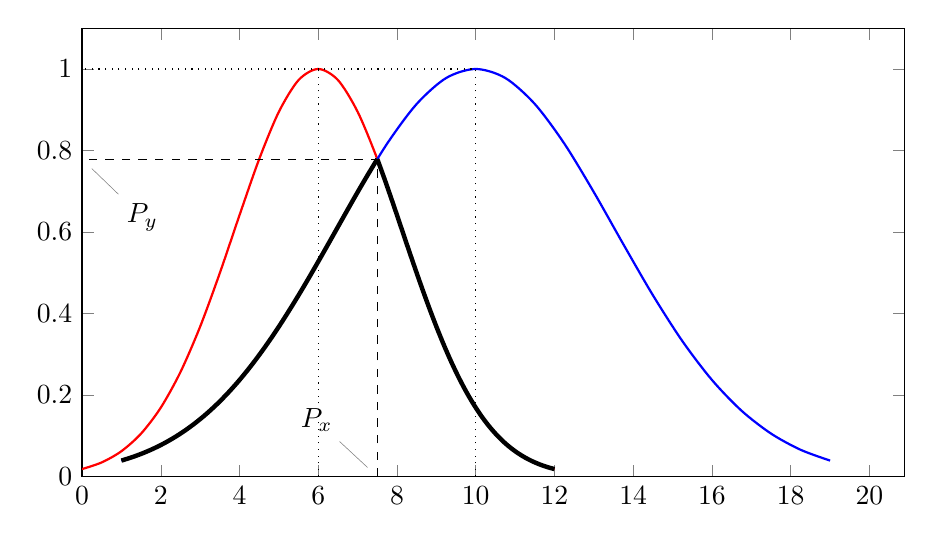
\begin{tikzpicture}
	\begin{axis}[x=.5cm,xmin=0,ymin=0]
	\addplot[mark=none,smooth,red,thick] expression[domain=0:12]{exp(((x-6)^2)/(-9))};
	\addplot[mark=none,smooth,blue,thick] expression[domain=1:19]{exp(((x-10)^2)/(-25))};
	\addplot[mark=none,smooth,ultra thick] expression[domain=7.5:12]{exp(((x-6)^2)/(-9))};
	\addplot[mark=none,smooth,ultra thick] expression[domain=1:7.5]{exp(((x-10)^2)/(-25))};
	\addplot[dotted,mark=none]coordinates{(6,0)(6,1)};
	\addplot[dotted,mark=none]coordinates{(10,0)(10,1)(0,1)};
	\addplot[dashed,mark=none]coordinates{(7.5,0)(7.5,0.7788)(0,0.7788)};
	\node[pin=-45:{$P_y$}] at (axis cs:0,0.7788) {};
	\node[pin=135:{$P_x$}] at (axis cs:7.5,0) {};
	\end{axis}
\end{tikzpicture}
%	\end{spacing}

\begin{tikzpicture}
\begin{axis}
\addplot[color=red]{exp(x)};
\end{axis}
\end{tikzpicture}
%Here ends the furst plot
\hskip 5pt
%Here begins the 3d plot
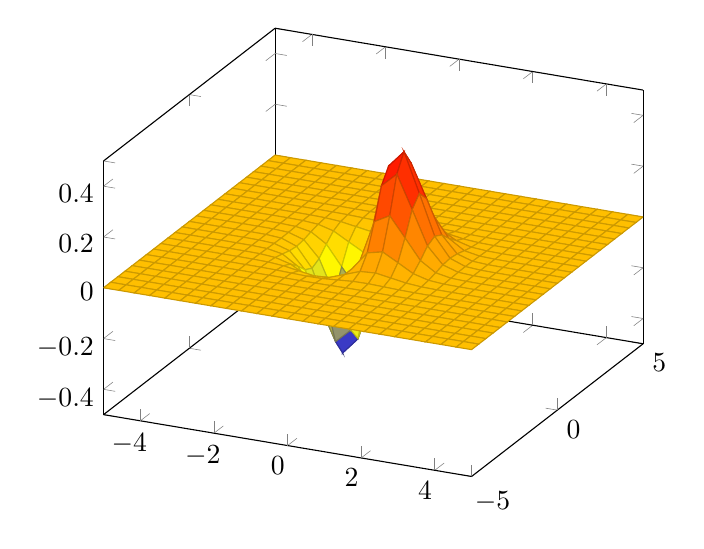
\begin{tikzpicture}
\begin{axis}
\addplot3[surf,]
{exp(-x^2-y^2)*x};
\end{axis}
\end{tikzpicture}
文字环绕 文字环绕文字环绕文字环绕文字环绕文字环绕文字环绕文字环绕
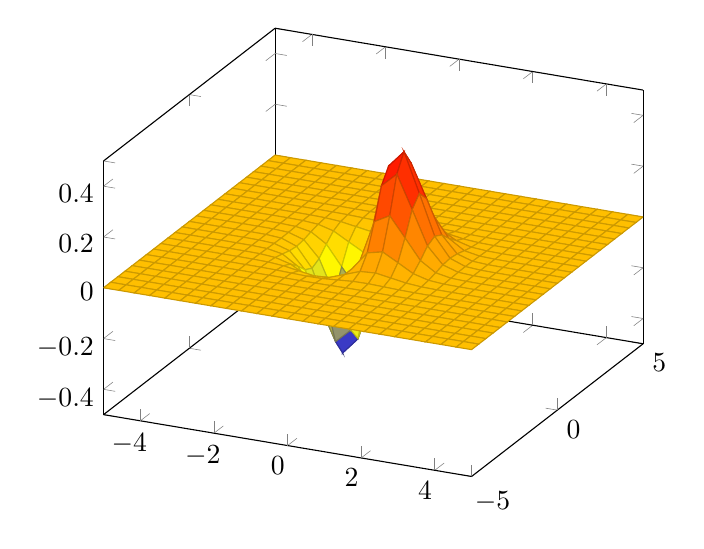
\begin{tikzpicture}
\begin{axis}
\addplot3[surf,]
{exp(-x^2-y^2)*x};
\end{axis}
\end{tikzpicture}
\begin{tikzpicture}
%画直角坐标系
\draw[thick,-latex](-3,0)--(3,0)node[below]{$ x $};
\draw[thick,-latex](0,-3)--(0,3)node[left]{$ y $};
%画椭圆
\draw[thick,blue](2,0)arc(0:360:2 and 1.732);
%定义坐标
\coordinate[label=above:$ P $](P)at(2*cos 60,1.732*sin 60);
\coordinate[label=below:$ F_1 $](f1)at(-1,0);
\coordinate[label=below:$ F_2 $](f2)at(1,0);
\coordinate[label=225:$ B $](B)at(-2,0);
\coordinate[label=-45:$ A $](A)at(2,0);
\coordinate[label=45:$ N $](N)at(0,2);
\coordinate[label=35:$ H $](H)at($ (N)!(f2)!(P) $);
%找交点
\tkzInterLL(f1,P)(f2,H) \tkzGetPoint{G}
\coordinate[label=45:$ G $](g)at(G);
%画切线
\draw[thick,blue,domain=-1:3]plot(\x,{2-(1/2)*\x});
%连线
\draw[thick,blue](B)--(H)(f1)--(g)(f2)--(g)(A)--(H)(f2)--(P);
\draw[thick,blue,dashed](0,0)--(H);
%标记原点
\node at (-.2,-.2){$ O $};
%画直角符号
\draw[thick,red]($ (H)!0.15!(g) $)coordinate(c1)--($ (c1)!1!-90:(H) $)coordinate(c2)--($ (c2)!1!-90:(c1) $);
%画点
\foreach \x in {P,f1,f2,B,A,N,H,g}
\shade[ball color=red](\x)circle(2pt);
\end{tikzpicture}
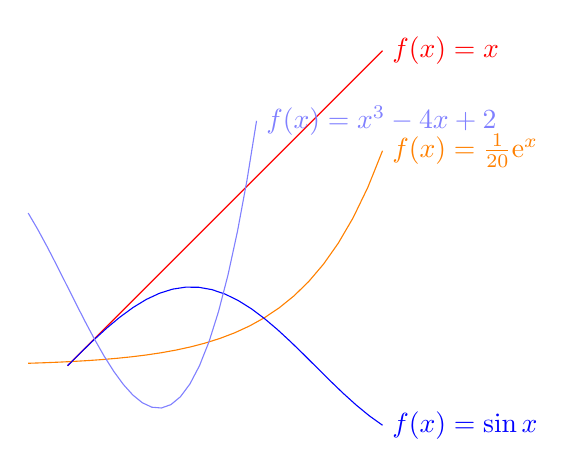
\begin{tikzpicture}[domain=0:4]
\tkzInit[xmax=4.2,ymax=3.2,xmin=-1.2,ymin=-1.2,xstep=1]
%\tkzGrid
\tkzAxeXY
\draw[color=red] plot (\x,\x) node[right] {$f(x)=x$};
\draw[color=orange,domain=-0.5:4] plot (\x,{0.05*exp(\x)}) node[right] {$f(x)=\frac{1}{20}\mathrm e^x$};
\draw[color=blue,domain=0:4] plot (\x,{sin(\x r)}) node[right] {$f(x)=\sin x$};
\draw[color=blue!50,x=1cm,y=0.5cm,domain=-0.5:2.4] plot (\x, {(\x)^3-4*(\x)+2}) node[right] {$f(x)=x^3-4x+2$};
\end{tikzpicture}

%\clearpage
\vspace{-6.5cm}
\setlength{\marginparsep}{1.7cm}
\iftagged{ans}{}{\putzdx} %%装订线--奇页数
\vspace{1cm}
\end{document}